\documentclass{report}
\usepackage[francais]{babel}
\usepackage[utf8]{inputenc}
\usepackage[T1]{fontenc}
\usepackage{amssymb}
\usepackage{graphicx}
\newcommand{\HRule}{\rule{\linewidth}{0.5mm}}
\bibliographystyle{unsrt}
\begin{document}

\begin{titlepage}

\begin{center}

\textsc{\LARGE \'Etat de l'art}\\[1.5cm]

\textsc{\Large EPITA}\\[0.5cm]

\HRule \\[0.4cm]
{ \huge \bfseries MLEA - Empreintes digitales}\\[0.4cm]

\HRule \\[1.5cm]

\large
\emph{Auteurs:}\\
Thomas \textsc{Badie}\\
Victor \textsc{Lenoir}\\
David \textsc{Moreira}\\
Pierre \textsc{Parutto}\\

\vfill

% Bottom of the page
{\large \today}

\end{center}

\end{titlepage}
%\maketitle
\newpage
\tableofcontents
\newpage

\chapter{Introduction}
La reconnaissance d'empreintes digitales consiste en une
reconnaissance d'un motif (empreinte sur le doigt) permettant
d'identifier le possesseur de cette empreinte. Il y a deux types
d'applications utilisant la reconnaissance d'empreintes :

\begin{description}
\item[Vérification] Une personne décline son identité et on vérifie
  que c'est vrai en comparant l'empreinte sur le doigt avec celle dans
  la base et on répond oui ou non ;
\item[Identification] On n'a aucun indice à l'avance sur l'identité du
  possesseur de l'empreinte. Il faut donc comparer l'image à toutes
  celles de la base.
\end{description}

La phase d'acquisition, généralement commune aux deux types
d'applications, correspond à l'enregistrement de l'empreinte dans la
base de donnée. Elle est généralement suivie par une algorithme de
validation de la qualité de l'enregistrement comme le montre la Figure
\ref{fig:schema-bloc-acq}.

\begin{figure}[H]
\centering
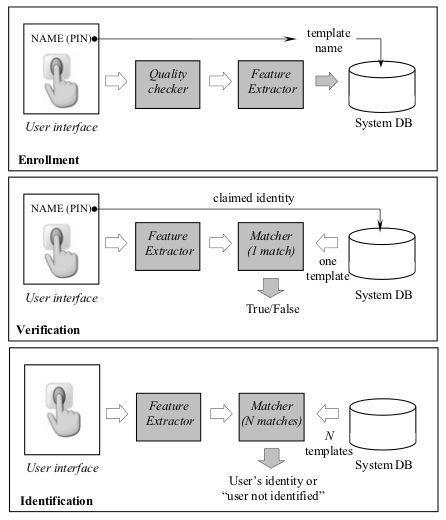
\includegraphics[scale=0.8]{three_way.png}
\caption{Schéma bloc de l'acquisition, de la vérification et de
  l'identification.}
\label{fig:schema-bloc-acq}
\end{figure}

Comme on peut le voir sur la Figure, l'image est ensuite transformée
en un modèle (\emph{template} en anglais) grâce à un extracteur de
caractéristiques (\emph{feature extractor} en anglais).

Dans le cas de la vérification, l'utilisateur entre son identifiant et
donne son empreinte. Celle-ci est transformée en un modèle compact.
On extrait le modèle lui correspondant dans la base de donnée, et un
comparateur est chargé de prendre la décision \og oui / non \fg.

Dans le cas de l'identification, c'est différent car il n'y a aucun
identifiant qui est donné et ce n'est plus un simple écart entre deux
modèles à calculer, mais un écart avec toutes les données de la base.
Les résultats possibles sont l'identité du possesseur des empreintes,
ou \og utilisateur non identifié \fg.

Il y a différentes parties distinctes, et dans un premier temps, nous
allons traiter des problèmes liés à ce type de biométrie. Dans un
second temps, nous allons traiter deux méthodes permettant la
vérification ou l'identification d'individu. La première de ces
méthodes et la méthode basé sur la corrélation entre deux empreintes
digitales. La seconde méthode se base sur les défauts que peuvent
présenter les empreintes digitales.


%%% Local Variables:
%%% mode: latex
%%% TeX-master: "../mlea"
%%% End:


\section{Problèmes liés à la biométrie}

Il y a divers problèmes liés à cette biométrie, notamment lors de
l'acquisition. Il y a principalement deux moyens d'effectuer ce
processus \emph{off-line}, c'est à dire la méthode ancestrale avec de
l'encre sur le doigt et apposé sur du papier, et \emph{live} qui
correspond à utiliser un scanner numérique. Pour assurer une
compatibilité entre ses deux méthodes d'acquisition, le ``US Criminal
Justice Information Services'' a présenté un ensemble de
spécifications pour fixer la qualité et le format des images (voir
annexes F et G de \cite{nla.cat-vn4185009}).

Bien que la méthode à l'encre ait commencé à être utilisé il y a très
longtemps (plus d'une trentaine d'année) elle est toujours utilisée
dans des applications à caractères légales. Les bases de données des
agences américaines de sécurités contiennent des données ayant été
acquises par les deux méthodes, ce qui signifie que les algorithmes
travaillant sur ces bases doivent être capables de les traiter
indépendemment.

Un des avantages d'utiliser l'acquisition avec l'encre est que l'on
peut enregistrer tout le doigt en effectuant un mouvement rotatif en
partant avec son doigt perpendiculaire d'un côté pour aller à
perpendiculaire de l'autre, ce qui n'est pas possible avec un scanner
numérique.

En contrepartie, il est possible, en fonction de comment est placée
l'encre sur le doigt, de laisser des zones de vide ou alors trop
pleine.

Du côté des acquisitions numériques, la plupart des appareils peuvent
se classer dans trois catégories différentes :

\begin{description}
\item[Optiques] le plus vieux et le plus utilisé des techniques
  d'acquisitions actuelles. Cette méthode fonctionne avec un prisme en
  verre. L'utilisateur doit mettre son doigt en haut de ce prisme est
  l'acquisition se fait ainsi.

  Ce type d'appareil a l'avantage de faire des images de bonnes
  qualités et d'avoir une grande surface du doigt enregistrée. Par
  contre, on ne peut pas miniaturiser cet appareil ;
\item[Ultrasons] il s'agit d'envoyer des ultrasons sur le doigt et de
  récupérer l'écho. Il est ainsi possible de dessiner la structure de
  l'empreinte digitale. Les images sont de bonne qualités, mais le
  système est onéreux ;
\item[Semi conducteurs] il y a quatre principales méthodes :
  thermique, capacitive, par champs électrique et piezoélectrique.  Il
  s'agit de toucher une carte en silice où chaque pixel est un petit
  capteur.
\end{description}

À présent que nous avons présenté les différentes manières de faire
l'acquisition, il nous faut à présent introduire quelques problèmes
communs à toutes les acquisitions. Il existe des variations en
fonction de l'état du doigt au moment de l'acquisition. Si celui-ci
est sec ou humide, l'image finale est différente.

Il existe aussi des problèmes de translation, de rotation ainsi que
des problèmes d'élasticité du doigt.


%%% Local Variables:
%%% mode: latex
%%% TeX-master: "../mlea"
%%% End:


\chapter{Correlation-based}
\chapter{Minuatiae Based}

La seconde méthode que nous allons traiter dans cet état de l'art est
la méthode basé sur l'extraction des minutia (ou minutiaes) sur les
empreintes digitales. Chaque empreinte comporte un certain nombre de
défaut, appelés minutiaes. Ces défauts sont unique pour chaque
individue. Cependant, il important de remarque que l'on a une chance
sur dix milliards d'avoir des minutia qui peuvent être assez
ressemblant pour être confondues. Les minutia sont des défauts de
l'empreinte digitales qui sont définie dès la naissance et qui sont
inchangeable durant la vie entière de l'individu.

Pour effectuer cette technique, il nous faut d'abord extraire un
maximum de ces défauts pour que la méthode puisse fonctionner d'une
façon optimale. Dans la seconde partie nous traiterons la méthode
permettant de valider si deux empreintes appartient bien au même
individu (et également au même doigt.)

\section{Détection des Minutiae}

Les minutiaes sont classés en divers types selon leurs spécification
et leurs formes géométrique et la typologies des lignes des
empreintes. L'A.N.S.I. (pour American Natiional Standards Insitute)

\chapter{Conclusion}

\bibliography{mlea}



\end{document}
